\documentclass[12pt,a4paper]{article}

\usepackage[utf8]{inputenc}
\usepackage[T1]{fontenc}
\usepackage{lmodern}
\usepackage[margin=2.5cm]{geometry}
\usepackage{amsmath}
\usepackage{booktabs}
\usepackage{graphicx}
\usepackage{hyperref}
\usepackage{float}
\usepackage{microtype}
\usepackage{parskip}
\usepackage{caption}
\usepackage{subcaption}
\usepackage{array}
\usepackage{longtable}
\usepackage{natbib}

\hypersetup{
  colorlinks=true,
  linkcolor=black,
  citecolor=black,
  urlcolor=blue
}

\title{Automated Sleep Staging of a Rodent EEG/EMG Dataset\\
       Using AccuSleePy: A Complete Analysis Pipeline}
\author{Collaboration Station Agent Team}
\date{March 2026}

\begin{document}

\maketitle

% ============================================================
\begin{abstract}
% ============================================================

This report describes the application of AccuSleePy, a Python-based automated
rodent sleep staging tool, to a publicly available mouse EEG/EMG dataset
\citep{Barger2019}. The dataset comprises 50 four-hour daytime recordings from
10 C57BL/6 mice (5 recordings per animal), sampled at 512 Hz with expert manual
sleep-stage labels provided as ground truth. Sleep staging was performed using
AccuSleePy's compact neural network model for 2.5-second epochs
(\texttt{ssann\_2(5)s.pth}). Distributional shift correction was applied to each
recording using a calibration set of 120 epochs per sleep stage (360 epochs
total), selected using evenly distributed sampling across each stage's occurrence
indices in the expert labels. Validation on held-out epochs (those not used in
calibration) yielded a mean Cohen's kappa of $0.9490 \pm 0.0148$ and a mean
accuracy of $97.25 \pm 0.72\%$, consistent with the benchmark reported in the
original AccuSleePy publication \citep{Barger2019}. No recordings were flagged
by quality control. Group-level sleep architecture showed a mean of
$34.53 \pm 7.76\%$ Wake, $54.64 \pm 6.16\%$ NREM, and $10.83 \pm 2.18\%$ REM
across all 50 recordings, with mean bout durations of $41.5 \pm 15.9$\,s
(Wake), $62.9 \pm 9.9$\,s (NREM), and $76.4 \pm 16.6$\,s (REM). The complete
analysis package, including scored label files, per-recording metrics, and
publication-quality figures, is provided alongside this report.

\end{abstract}

\tableofcontents
\newpage

% ============================================================
\section{Data}
% ============================================================

\subsection{Dataset}

The dataset is drawn from the Open Science Framework repository of Barger and
Frye \citep{BargerOSF2025} and is associated with the publication by Barger
et al.\ \citep{Barger2019}. The dataset consists of standard cortical EEG
and nuchal EMG recordings from 10 adult male C57BL/6 mice, each recorded
across five separate four-hour daytime sessions (50 recordings total). EEG and
EMG signals were sampled at 512 Hz. Expert manual sleep-stage labels are
provided at a resolution of 2.5 seconds per epoch (5,760 epochs per recording),
classified into three states: REM sleep (label~1), Wake (label~2), and NREM
sleep (label~3).

\subsection{Recording Specifications}

\begin{table}[H]
\centering
\caption{Dataset summary.}
\label{tab:dataset}
\begin{tabular}{ll}
\toprule
Property & Value \\
\midrule
Species & C57BL/6 mouse \\
Number of animals & 10 \\
Recordings per animal & 5 (daytime, 4-hour) \\
Total recordings & 50 \\
Sampling rate & 512\,Hz \\
Epoch length & 2.5\,s (1,280 samples/epoch) \\
Epochs per recording & 5,760 \\
Total epochs & 288,000 \\
EEG configuration & Standard cortical EEG \\
EMG configuration & Nuchal (neck) EMG \\
Label encoding & REM\,=\,1; Wake\,=\,2; NREM\,=\,3 \\
\bottomrule
\end{tabular}
\end{table}

\subsection{Label Distribution}

\begin{table}[H]
\centering
\caption{Expert manual label distribution across all 50 recordings (288,000 epochs total).}
\label{tab:labels}
\begin{tabular}{llrr}
\toprule
Label & Stage & Count & Percentage \\
\midrule
1 & REM  & 30,128  & 10.46\% \\
2 & Wake & 98,983  & 34.37\% \\
3 & NREM & 158,889 & 55.17\% \\
\midrule
  & \textbf{Total} & \textbf{288,000} & \textbf{100.00\%} \\
\bottomrule
\end{tabular}
\end{table}

% ============================================================
\section{Methods}
% ============================================================

\subsection{Data Loading}

All EEG and EMG signals are stored in Apache Parquet format
(\texttt{recording.parquet}; shape $7{,}372{,}800 \times 2$, dtype float64)
with columns \texttt{eeg} and \texttt{emg}. Expert manual labels are stored in
CSV format (\texttt{labels.csv}; column \texttt{brain\_state}, dtype int64;
5,760 rows per recording). Signals were loaded using the pandas library;
label arrays were loaded with NumPy. Signal arrays were extracted as float64
NumPy arrays by selecting the respective column from the loaded DataFrame.

\subsection{Calibration}

AccuSleePy includes a distributional shift correction step (calibration) that
uses a small set of manually labeled epochs from the target recording to adjust
the model's decision boundaries before scoring \citep{Barger2019}. This step
is a core part of the standard AccuSleePy workflow and was applied to every
recording in this analysis.

For each recording, a calibration set of 360 epochs was constructed as follows.
For each of the three sleep stages (Wake, NREM, REM), all epoch indices carrying
that stage label in the expert labels were identified. A subset of 120 epochs
was then selected using evenly distributed positions:

\begin{verbatim}
np.linspace(0, len(stage_indices) - 1, 120, dtype=int)
\end{verbatim}

indexed into the array of per-stage occurrence indices. This distributes the
selected calibration epochs evenly across the full temporal span of each stage's
occurrences, capturing within-session variability in neural signal statistics.
The three per-stage sets (120 epochs each) were combined to form the final
360-epoch calibration set. The AccuSleePy built-in calibration function was
applied using these epochs and their corresponding expert labels before any
scoring took place. Calibration epoch indices were saved as companion files
alongside the predicted-label outputs and were excluded from all subsequent
validation comparisons.

\subsection{Scoring}

All epochs in each recording were scored using AccuSleePy's pre-trained
2.5-second model (\texttt{ssann\_2(5)s.pth}) applied after calibration.
AccuSleePy produces one predicted label and one confidence score per epoch.
Output files were saved in CSV format (columns \texttt{brain\_state} and
\texttt{confidence\_score}; 5,760 rows per recording) to the
\texttt{outputs/predicted\_labels/} directory. No intermediate disk files are
created by AccuSleePy during scoring; all computations are performed in memory.

\subsection{Quality Control}

Quality control was applied to each recording's predicted label sequence using
the following criteria:

\begin{itemize}
  \item \textbf{Stage proportion plausibility:} a recording was flagged if Wake
    exceeded 80\%, REM exceeded 25\%, or NREM fell below 10\%.
  \item \textbf{Long unbroken runs:} a recording was flagged if any single stage
    persisted without interruption for more than 60 minutes.
  \item \textbf{Low-confidence epochs:} epochs with a confidence score
    $\leq 0.8$ were catalogued. For each recording, a CSV file listing all
    such epochs (columns: \texttt{epoch\_index}, \texttt{predicted\_label},
    \texttt{confidence\_score}) was written to the
    \texttt{low\_confidence\_epochs/} directory.
\end{itemize}

Flagged recordings were noted in \texttt{QC\_report.md} but were not excluded
from any analysis. The decision to exclude or retain flagged recordings is left
to the researcher.

\subsection{Validation Against Expert Labels}

For each recording, the predicted label sequence was compared to the expert
manual labels on the set of held-out epochs (all epochs not included in the
calibration set; 5,400 per recording on average). The following metrics were
computed using shared utilities in \texttt{scripts/utils/metrics.py}:

\begin{itemize}
  \item \textbf{Cohen's kappa} --- the primary validation metric; accounts for
    class imbalance.
  \item \textbf{Overall accuracy} --- fraction of correctly classified
    held-out epochs.
  \item \textbf{Per-class precision, recall, and F1} for each of Wake, NREM,
    and REM.
  \item \textbf{Confusion matrix} --- $3 \times 3$ counts (rows = expert label;
    columns = predicted label) for each recording.
\end{itemize}

Aggregate statistics (mean $\pm$ SD across all 50 recordings) were computed for
kappa, accuracy, and per-class F1.

\subsection{Descriptive Sleep Metrics}

The following metrics were computed per recording from the predicted label
sequence (not from expert labels):

\begin{itemize}
  \item \textbf{Stage proportions:} percentage of total epochs classified as
    Wake, NREM, and REM.
  \item \textbf{Bout analysis:} a bout is defined as a continuous, uninterrupted
    run of epochs assigned to the same stage. For each stage, mean bout duration,
    maximum bout duration, and total bout count were computed. Durations are
    expressed in seconds (epoch length $= 2.5$\,s).
  \item \textbf{State transition probability matrix:} for each pair of stages
    $(i, j)$, the proportion of all transitions out of stage $i$ that lead to
    stage $j$. Rows are normalized to sum to 1.
  \item \textbf{Low-confidence epoch summary:} per-recording count and
    percentage of epochs with confidence score $\leq 0.8$.
\end{itemize}

All metrics were saved to \texttt{outputs/sleep\_metrics.csv}
(50 rows $\times$ 26 columns).

\subsection{Software}

\begin{table}[H]
\centering
\caption{Software environment.}
\label{tab:software}
\begin{tabular}{ll}
\toprule
Component & Version \\
\midrule
Python   & 3.11.9 \\
AccuSleePy & 0.12.0 \\
NumPy    & 2.4.3 \\
SciPy    & 1.17.1 \\
pandas   & 2.3.3 \\
matplotlib & 3.10.8 \\
PyTorch  & 2.10.0 \\
torchvision & 0.25.0 \\
\bottomrule
\end{tabular}
\end{table}

Full pinned dependency versions are available in \texttt{requirements.txt}.

% ============================================================
\section{Results}
% ============================================================

\subsection{Pipeline Validation}

Validation is presented as a technical quality check confirming that the
AccuSleePy pipeline executed correctly on this dataset. It is not the primary
scientific deliverable of this analysis.

Predicted labels were compared to expert manual labels on held-out epochs for
all 50 recordings. The aggregate 3$\times$3 confusion matrix (summed across all
recordings, normalized to row percentages) is shown in
Figure~\ref{fig:confusion}. The distribution of per-recording Cohen's kappa
values is shown in Figure~\ref{fig:kappa}.

\begin{figure}[H]
  \centering
  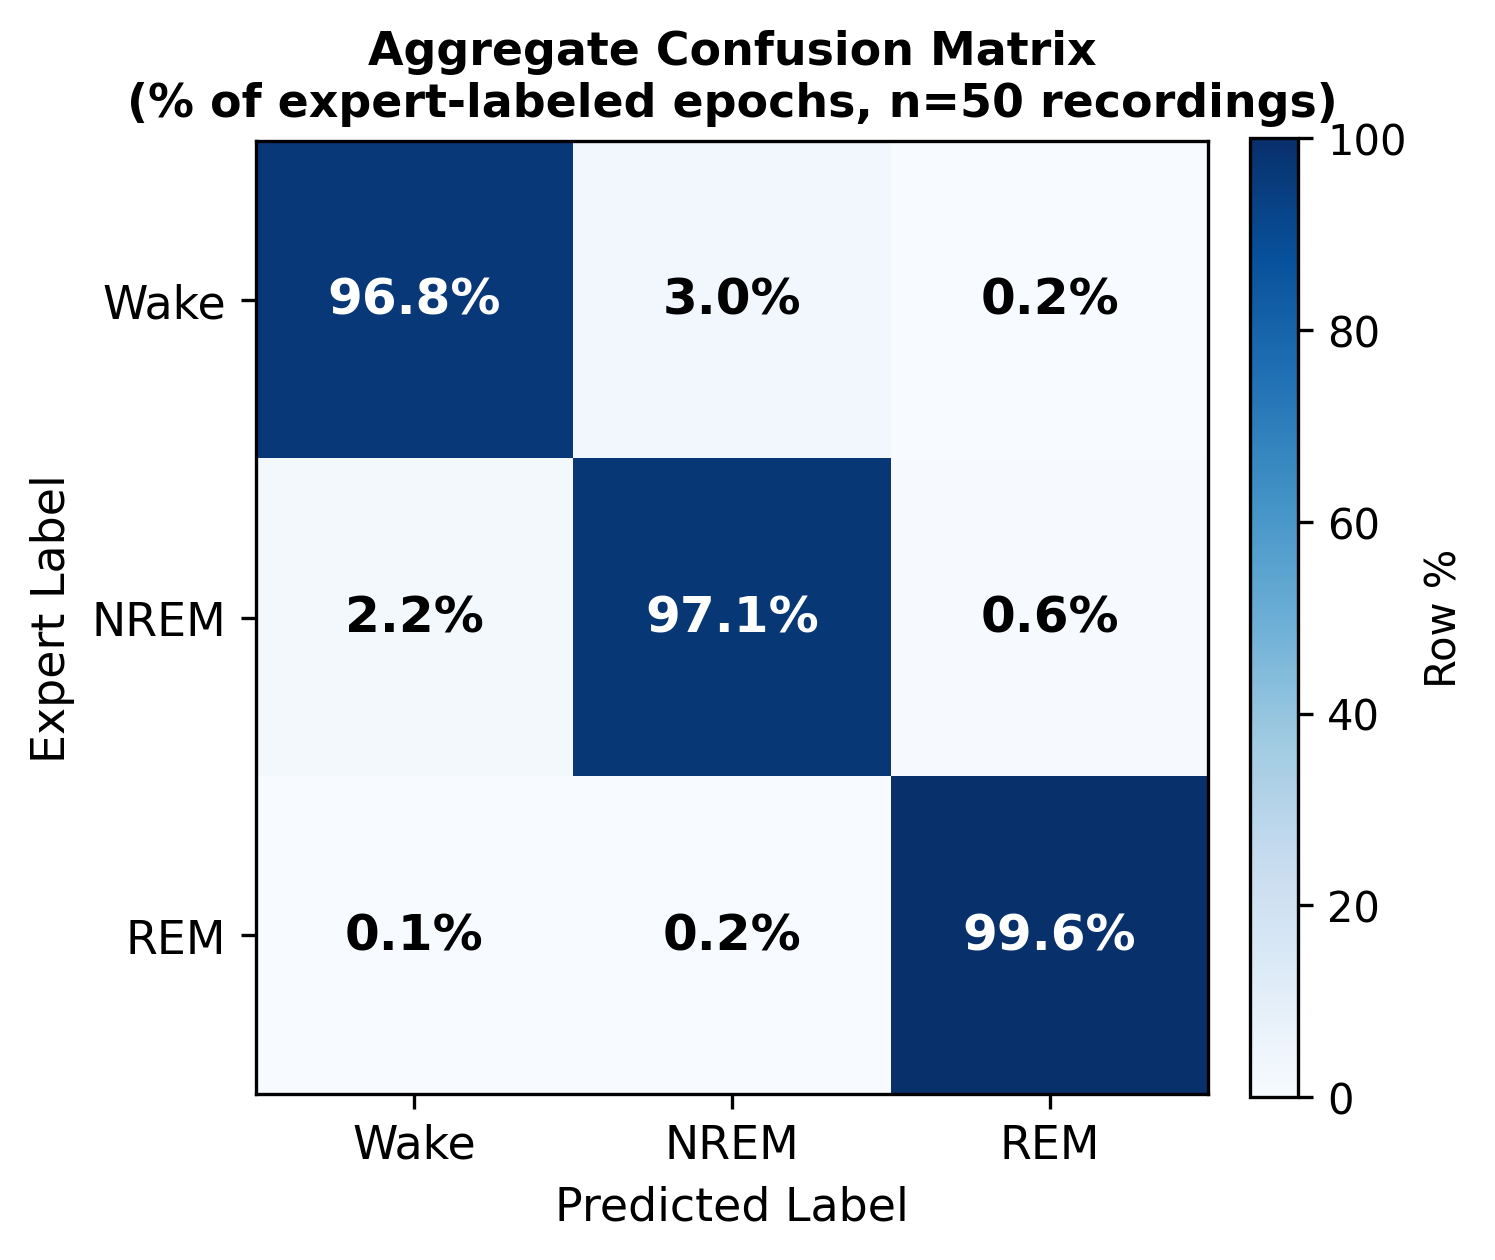
\includegraphics[width=0.55\textwidth]{../figures/validation/confusion_matrix.png}
  \caption{Aggregate confusion matrix across all 50 recordings (row-normalized to
    percentages). Rows represent expert labels; columns represent AccuSleePy
    predicted labels. Stage order: Wake, NREM, REM.}
  \label{fig:confusion}
\end{figure}

\begin{figure}[H]
  \centering
  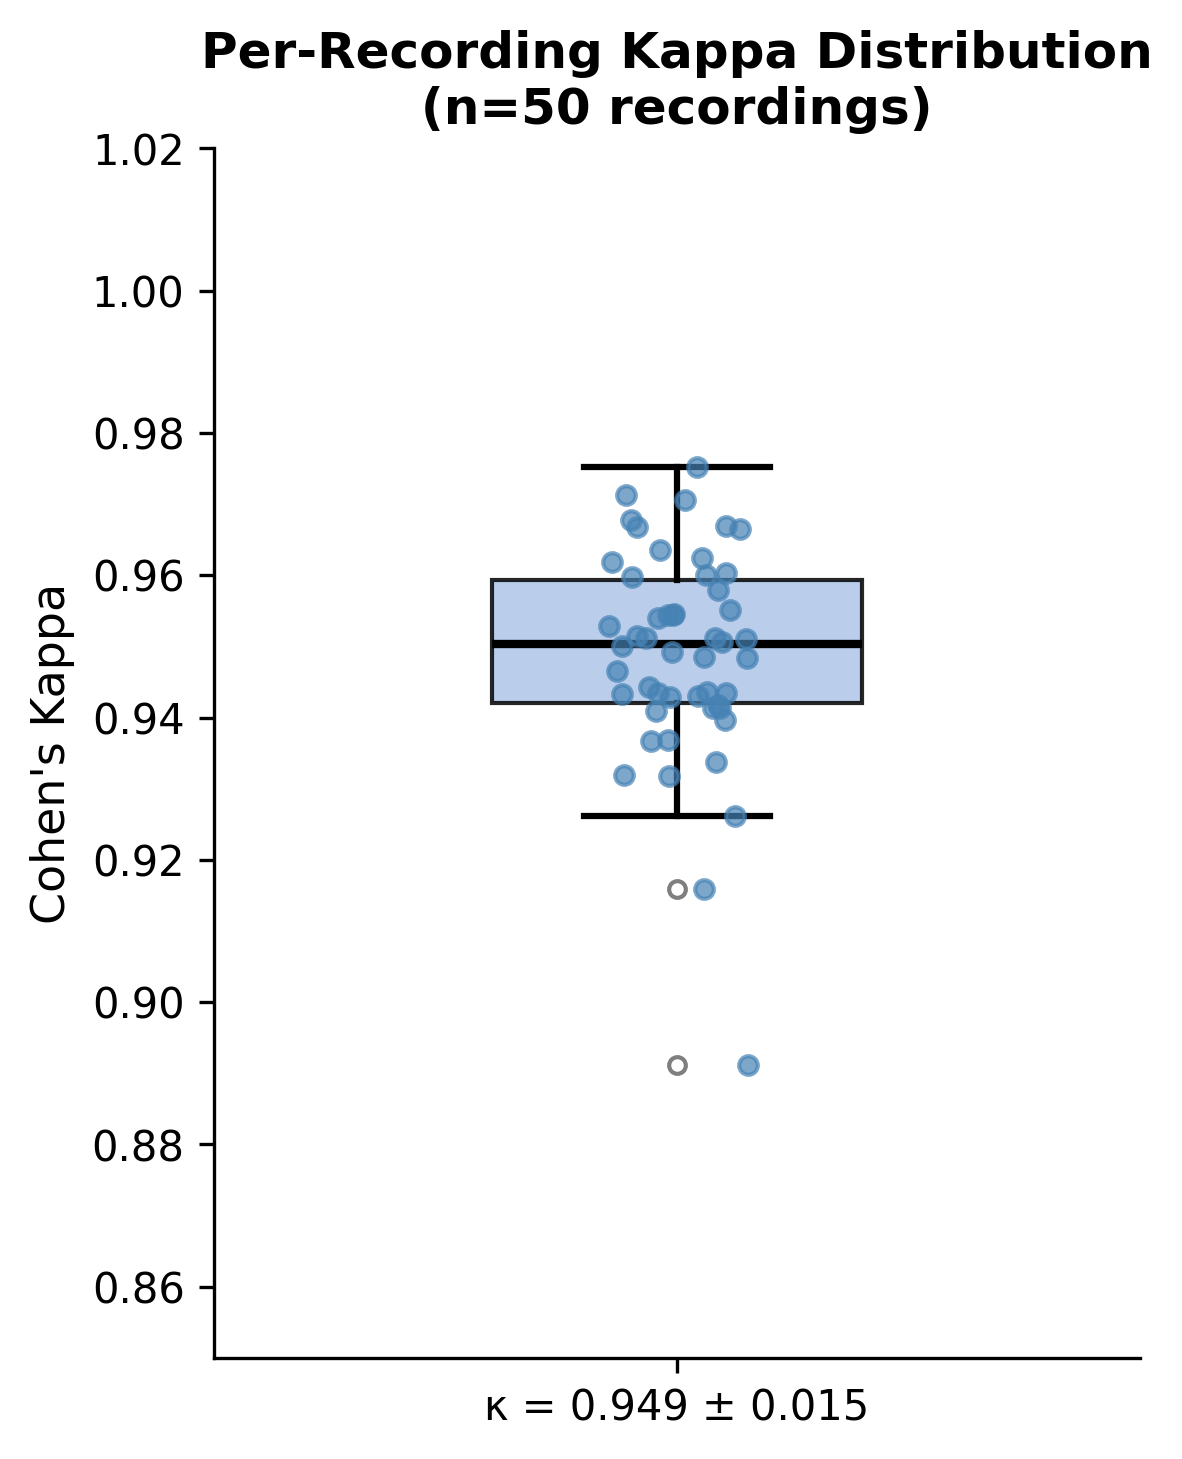
\includegraphics[width=0.5\textwidth]{../figures/validation/kappa_distribution.png}
  \caption{Distribution of Cohen's kappa values across all 50 recordings.
    Box shows median and interquartile range; individual recording values are
    overlaid.}
  \label{fig:kappa}
\end{figure}

\begin{table}[H]
\centering
\caption{Aggregate validation metrics (mean $\pm$ SD across 50 recordings). Calibration
  epochs (360 per recording) were excluded from all comparisons.}
\label{tab:validation}
\begin{tabular}{lll}
\toprule
Metric & Mean & SD \\
\midrule
Cohen's kappa & 0.9490 & 0.0148 \\
Accuracy      & 97.25\% & 0.72\% \\
\midrule
Wake precision  & 95.90\% & --- \\
Wake recall     & 96.60\% & --- \\
Wake F1         & 0.9623  & 0.0174 \\
NREM precision  & 98.12\% & --- \\
NREM recall     & 97.17\% & --- \\
NREM F1         & 0.9763  & 0.0050 \\
REM precision   & 95.54\% & --- \\
REM recall      & 99.64\% & --- \\
REM F1          & 0.9754  & 0.0093 \\
\bottomrule
\end{tabular}
\end{table}

The mean accuracy of 97.25\% is consistent with the benchmark of approximately
96.8\% reported in the original AccuSleePy publication for the same dataset and
pre-trained model \citep{Barger2019}, confirming that the pipeline is executing
as expected.

\subsection{Quality Control Summary}

Zero of 50 recordings were flagged by any quality control criterion. No
recording exceeded the Wake $>$ 80\% or REM $>$ 25\% thresholds, and no
recording had NREM below 10\%. No unbroken stage runs exceeding 60 minutes were
detected.

A total of 481 low-confidence epochs (confidence score $\leq 0.8$) were
identified across all 50 recordings, representing a mean of 0.167\% of total
epochs per recording. Per-recording low-confidence epoch lists are available in
the \texttt{low\_confidence\_epochs/} directory for manual review if desired.
No recordings were excluded from the analysis.

\subsection{Sleep Architecture}

The following results characterize the group-level sleep architecture of the
10 animals across all 50 recordings. These metrics constitute the primary
analytical deliverable of the AccuSleePy analysis. All metrics are computed
from the AccuSleePy predicted labels.

\subsubsection{Stage Proportions}

Figure~\ref{fig:stage_pct} shows the group-level percentage of recording time
spent in each sleep stage. Each data point represents one animal's mean across
its 5 recordings. The three stages accounted for $34.53 \pm 7.76\%$ (Wake),
$54.64 \pm 6.16\%$ (NREM), and $10.83 \pm 2.18\%$ (REM) of total recording
time (mean $\pm$ SD across 10 animals).

\begin{figure}[H]
  \centering
  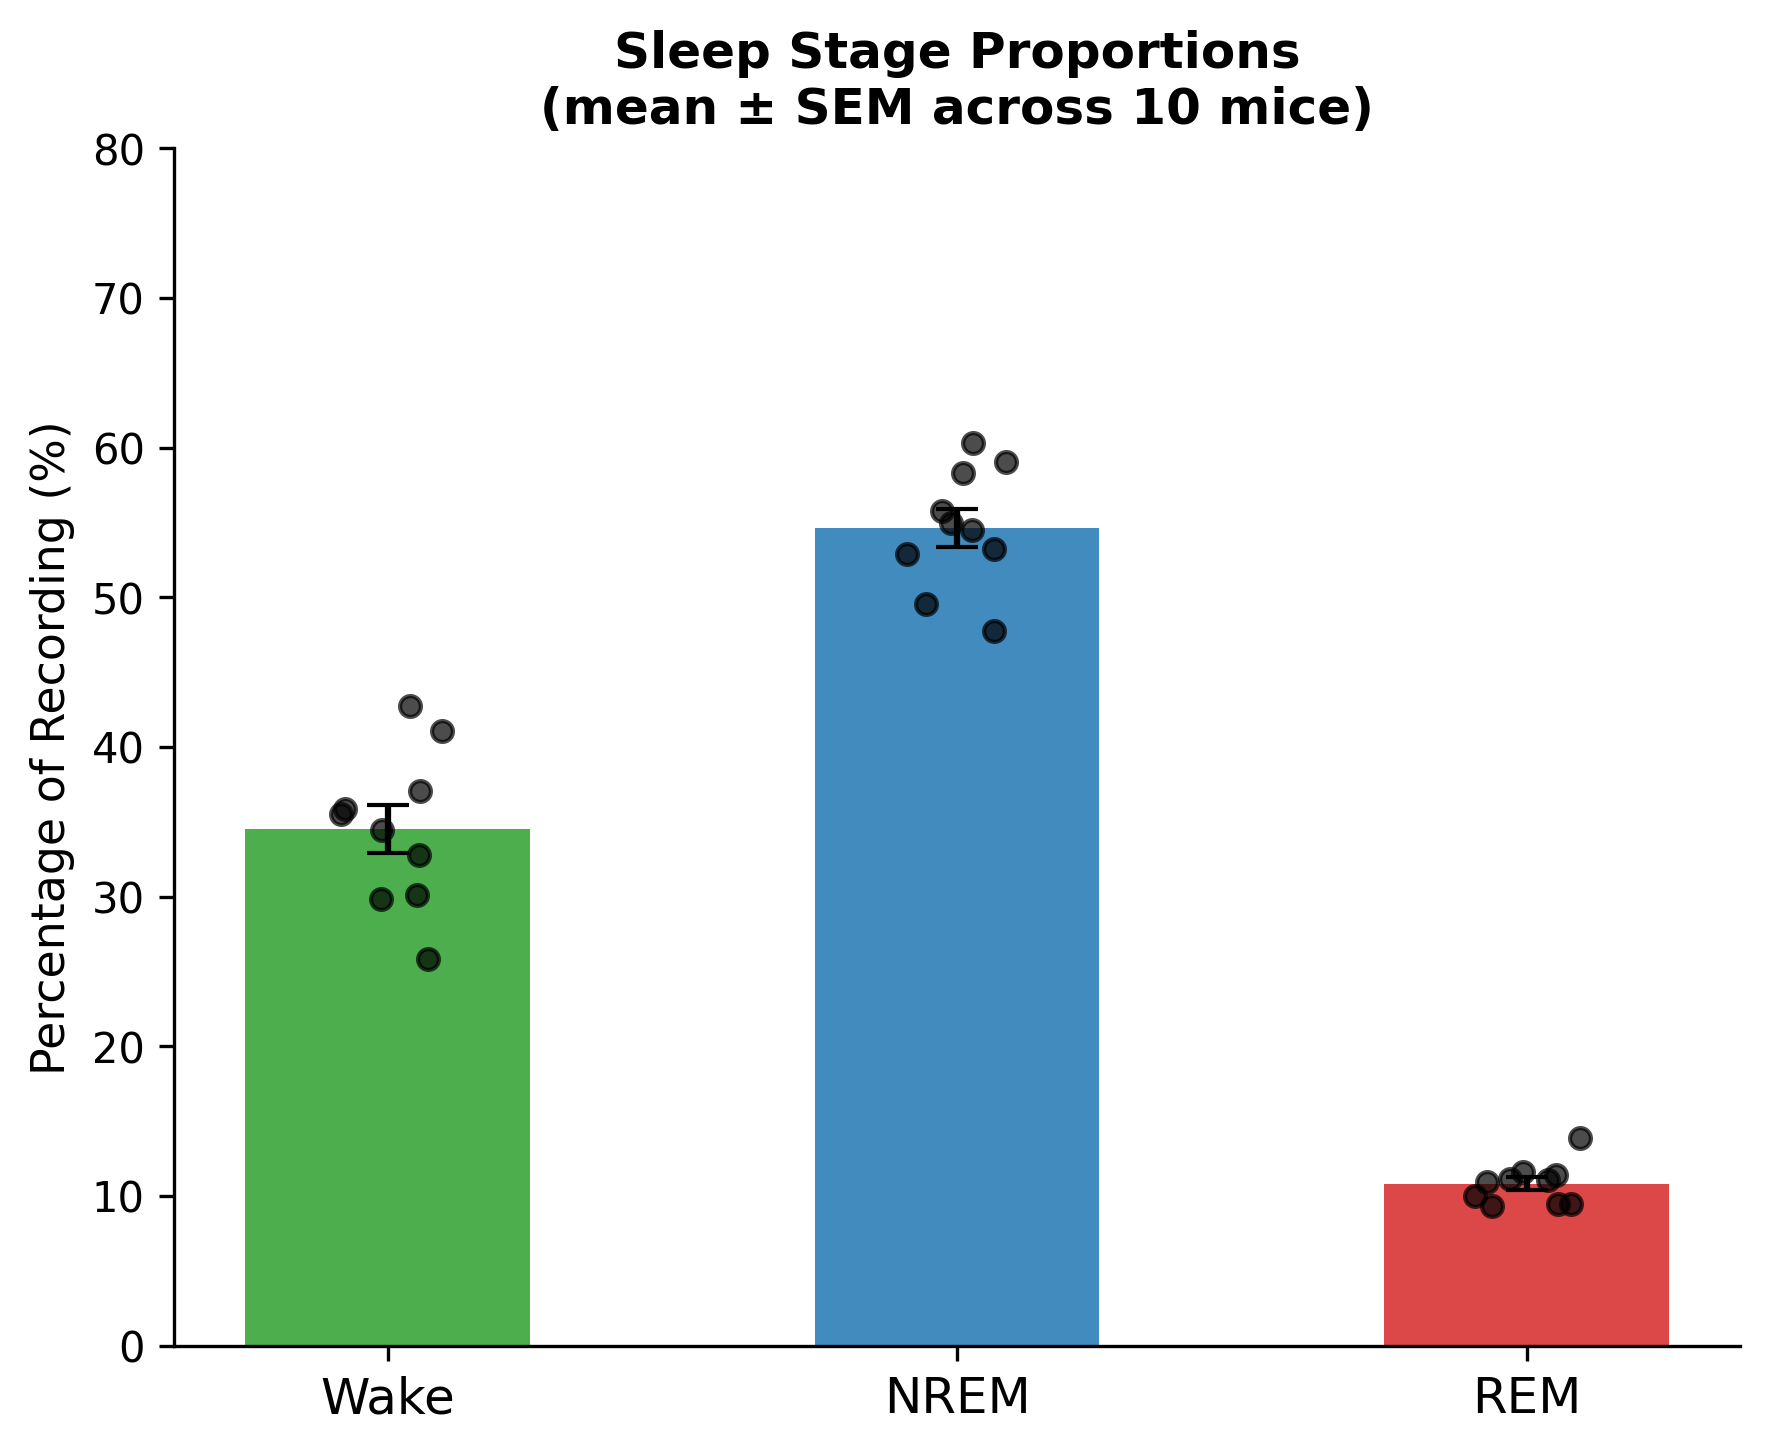
\includegraphics[width=0.6\textwidth]{../figures/stage_percentages/stage_percentages.png}
  \caption{Group-level stage proportions. Bars show mean $\pm$ SEM across 10
    animals. Individual animal means (averaged over 5 recordings per mouse)
    are overlaid as points. Wake\,=\,green, NREM\,=\,blue, REM\,=\,red.}
  \label{fig:stage_pct}
\end{figure}

\subsubsection{Bout Duration Analysis}

Figure~\ref{fig:bout} shows the distribution of mean bout duration per stage
across animals. Mean bout durations were $41.5 \pm 15.9$\,s (Wake),
$62.9 \pm 9.9$\,s (NREM), and $76.4 \pm 16.6$\,s (REM; mean $\pm$ SD
across 10 animals).

\begin{figure}[H]
  \centering
  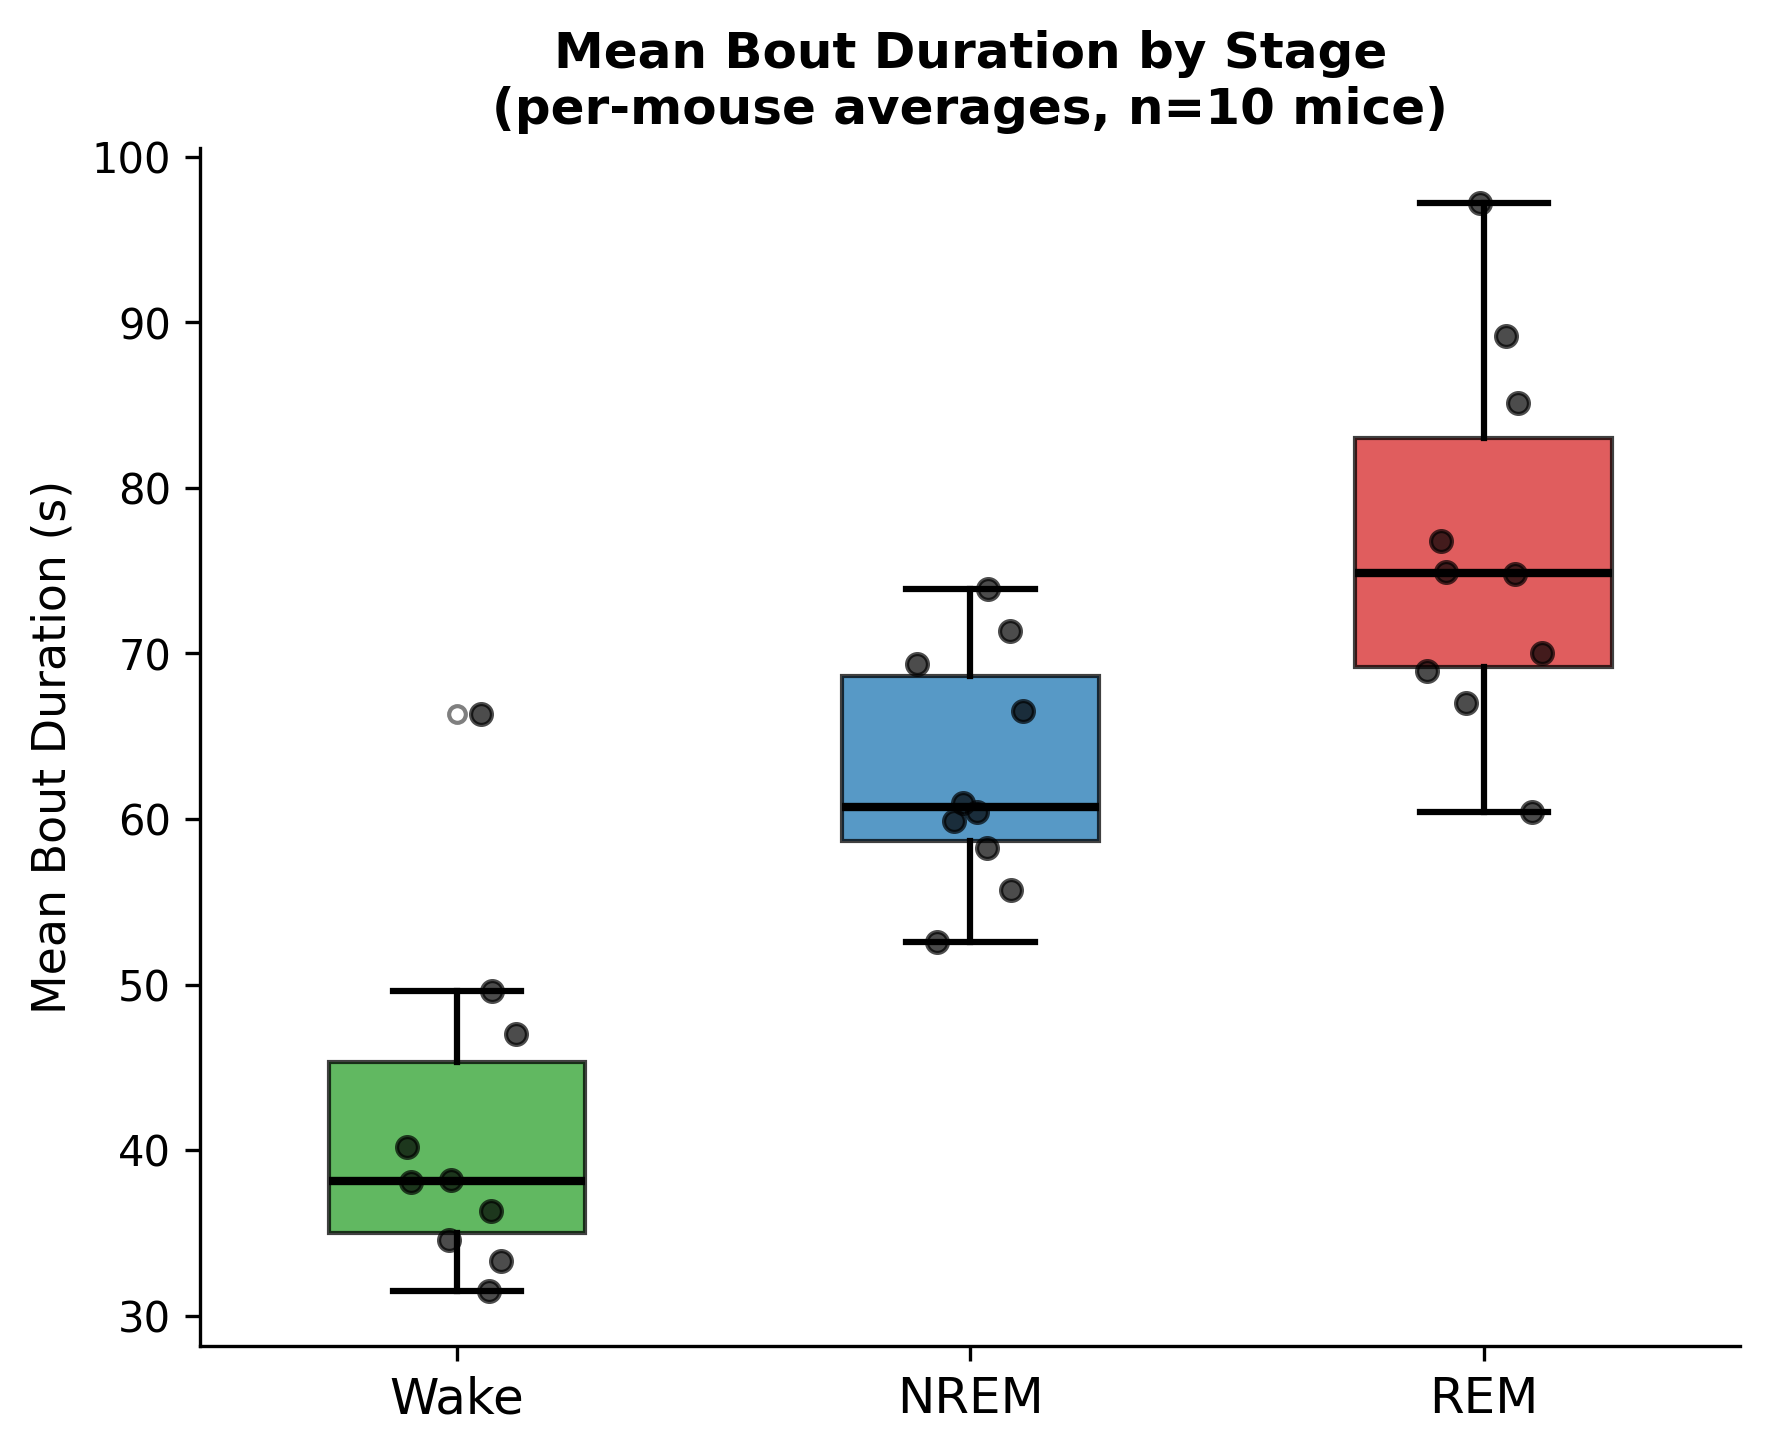
\includegraphics[width=0.6\textwidth]{../figures/bout_analysis/bout_duration.png}
  \caption{Mean bout duration (seconds) per stage across animals. Box plots show
    median and interquartile range; individual animal means are overlaid. Wake\,=\,green,
    NREM\,=\,blue, REM\,=\,red.}
  \label{fig:bout}
\end{figure}

\subsubsection{State Transition Probabilities}

Figure~\ref{fig:transitions} shows the mean state transition probability matrix
across all 50 recordings. Diagonal values (self-transitions, i.e., the
probability of remaining in the same stage at the next epoch boundary) are
large, reflecting the temporal stability of sleep stages. Off-diagonal entries
reveal the relative likelihood of transitions between stages.

\begin{figure}[H]
  \centering
  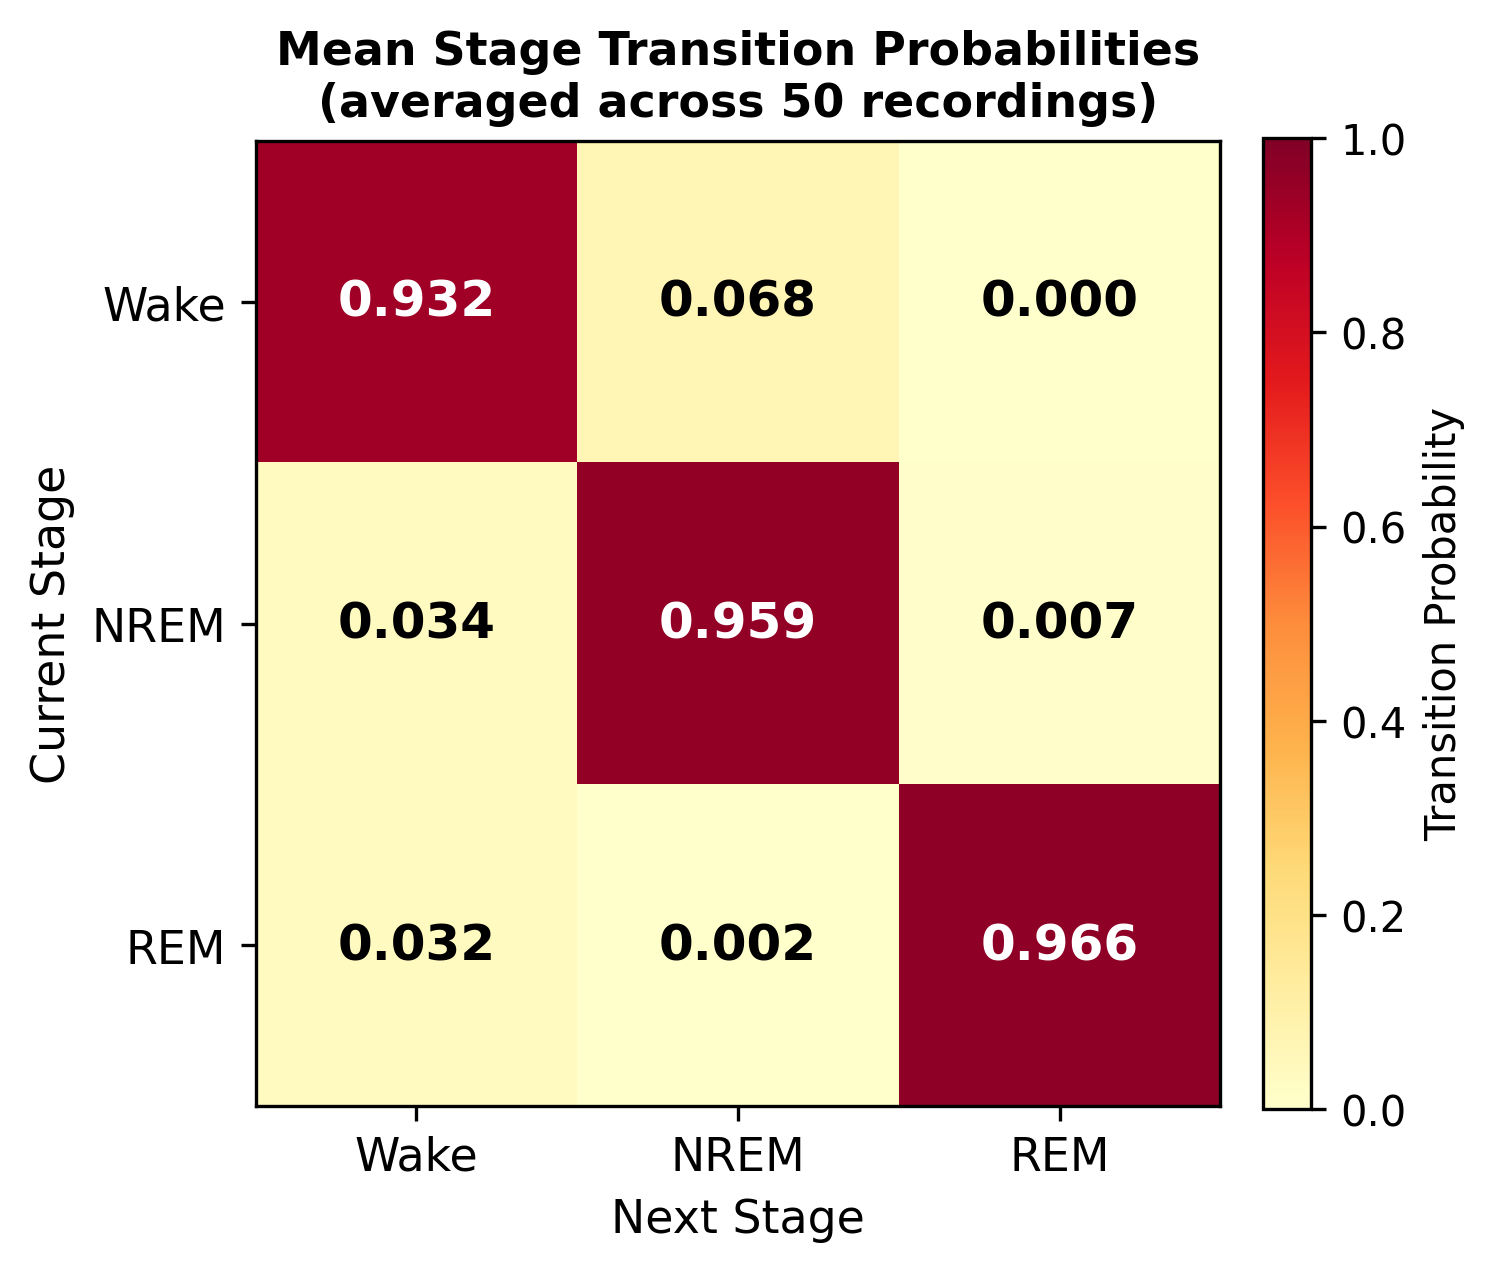
\includegraphics[width=0.5\textwidth]{../figures/transitions/transition_matrix.png}
  \caption{Mean state transition probability matrix (averaged across all 50
    recordings). Entry $(i,j)$ gives the probability that a transition out of
    stage $i$ leads to stage $j$. Rows are normalized to sum to 1.}
  \label{fig:transitions}
\end{figure}

\subsubsection{Representative Hypnograms}

Figures~\ref{fig:hyp1}--\ref{fig:hyp6} show the predicted sleep stage sequence
(hypnogram) for the Day\,1 recording of each of the six representative animals
(Mouse01--Mouse06). The $x$-axis represents time in hours; the $y$-axis
represents predicted stage. These hypnograms illustrate the typical alternating
pattern of Wake, NREM, and REM sleep characteristic of rodent daytime recordings.

\begin{figure}[H]
  \centering
  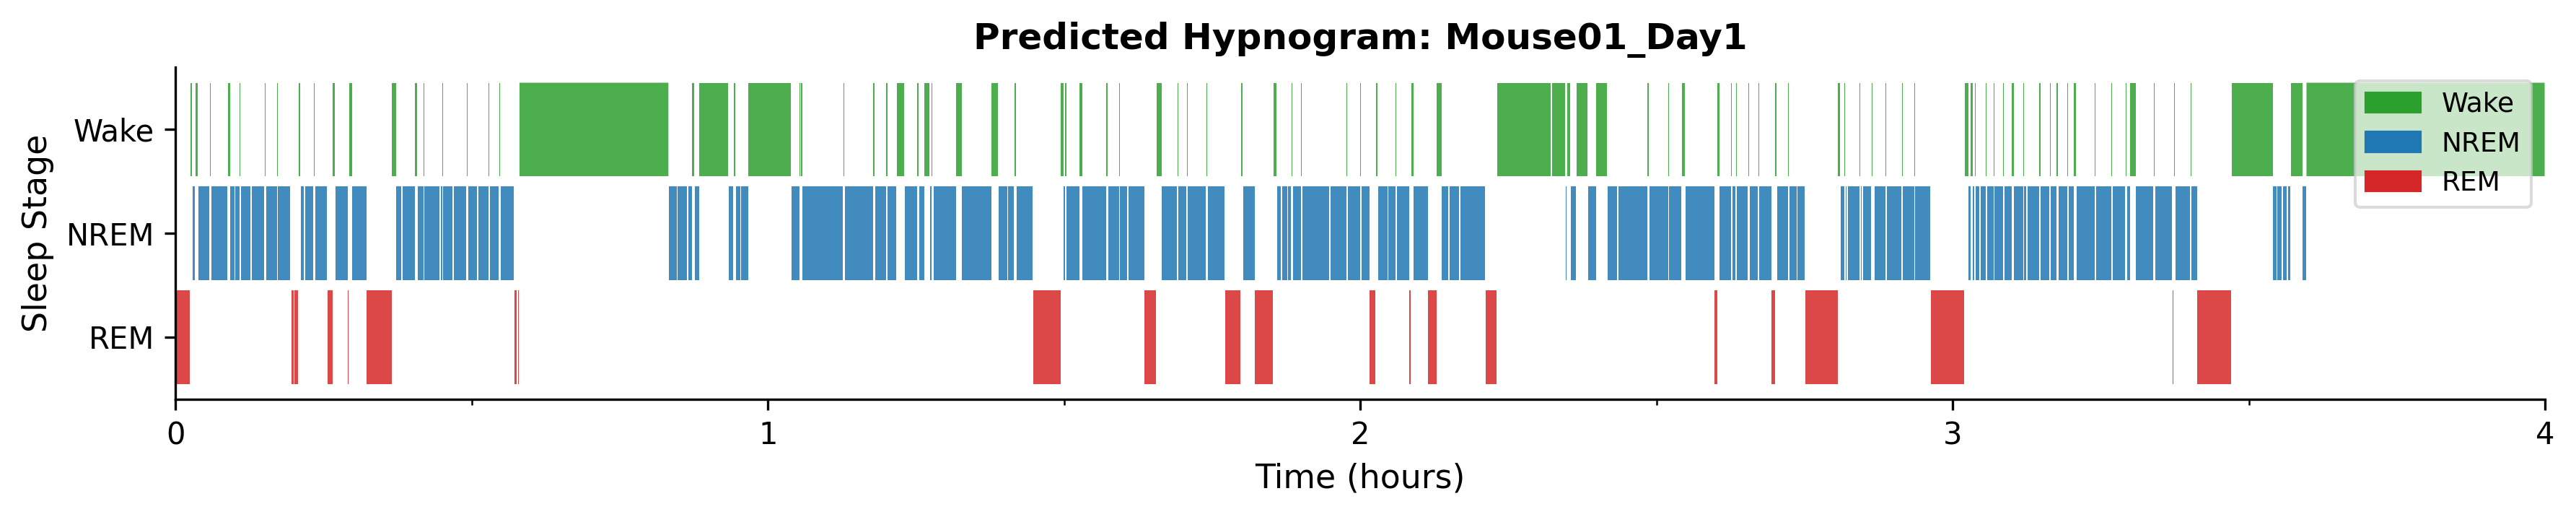
\includegraphics[width=\textwidth]{../figures/hypnograms/Mouse01_Day1_hypnogram.png}
  \caption{Predicted hypnogram: Mouse01, Day\,1 (4-hour recording).}
  \label{fig:hyp1}
\end{figure}

\begin{figure}[H]
  \centering
  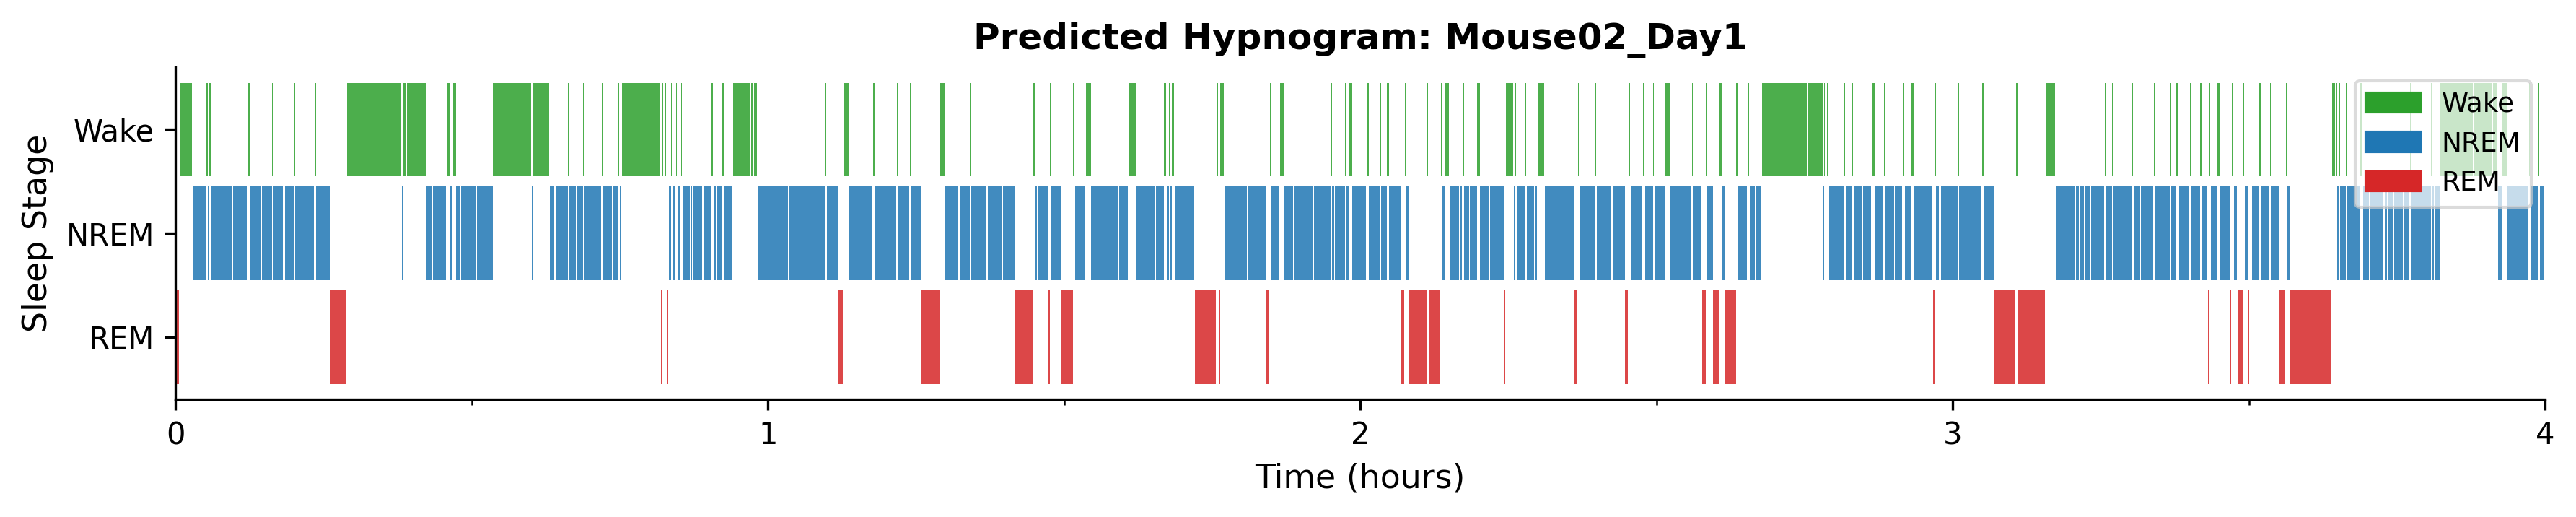
\includegraphics[width=\textwidth]{../figures/hypnograms/Mouse02_Day1_hypnogram.png}
  \caption{Predicted hypnogram: Mouse02, Day\,1.}
  \label{fig:hyp2}
\end{figure}

\begin{figure}[H]
  \centering
  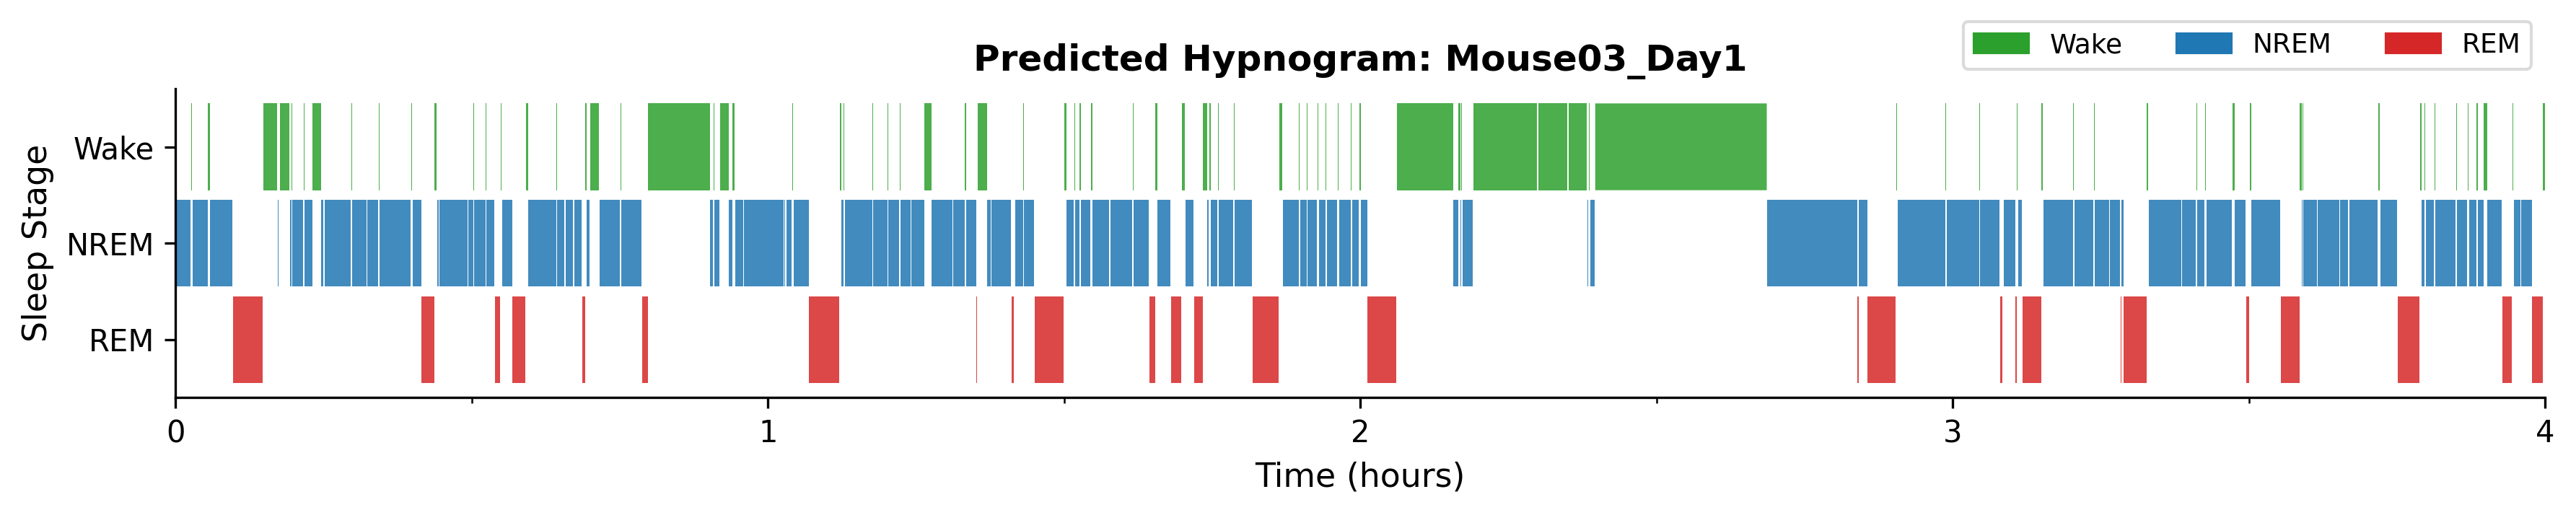
\includegraphics[width=\textwidth]{../figures/hypnograms/Mouse03_Day1_hypnogram.png}
  \caption{Predicted hypnogram: Mouse03, Day\,1.}
  \label{fig:hyp3}
\end{figure}

\begin{figure}[H]
  \centering
  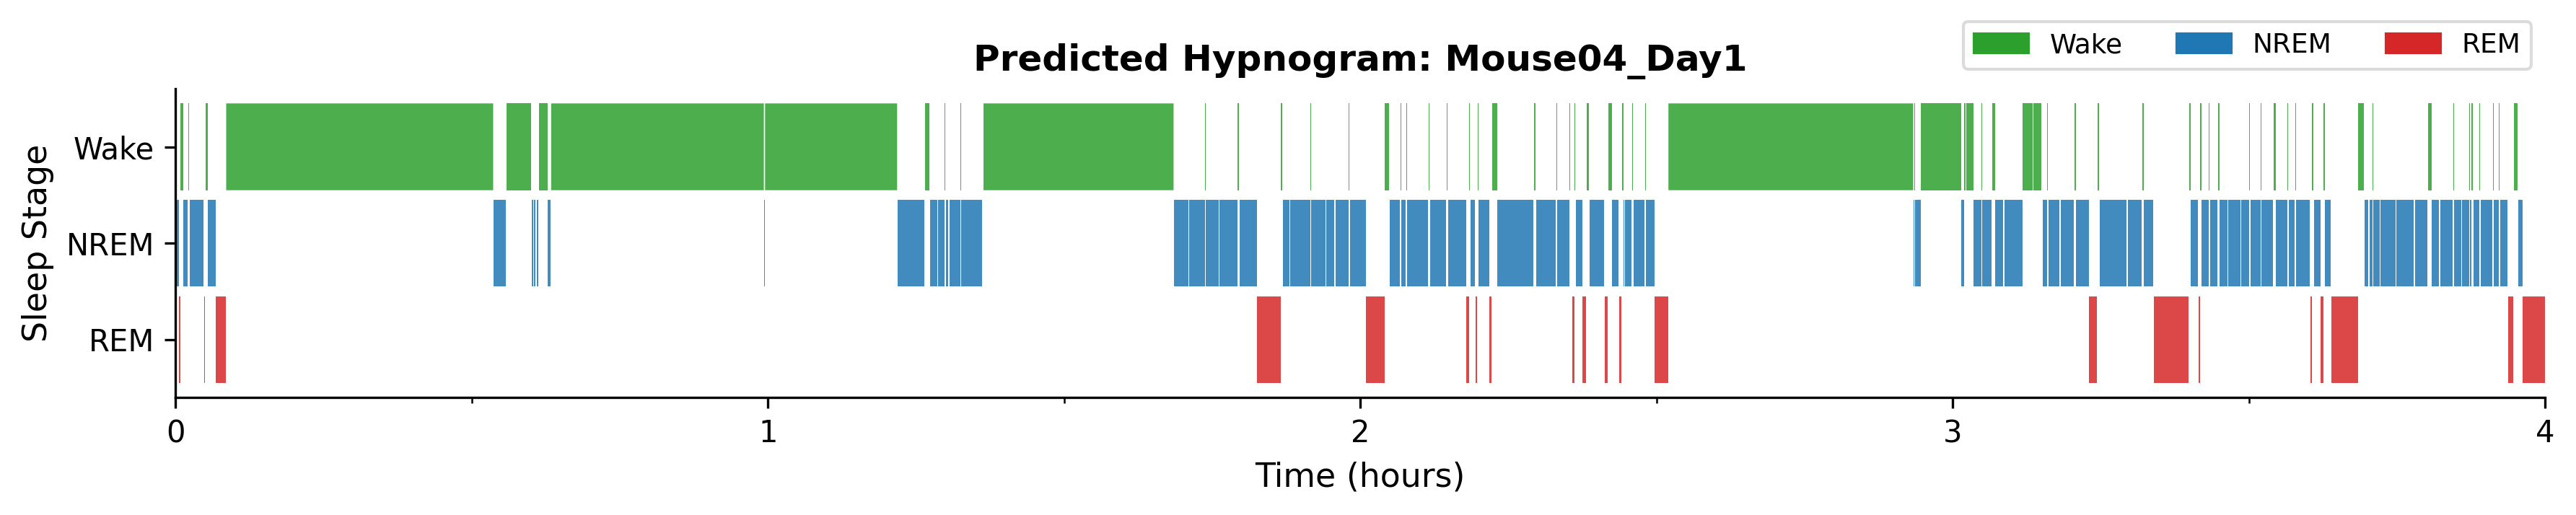
\includegraphics[width=\textwidth]{../figures/hypnograms/Mouse04_Day1_hypnogram.png}
  \caption{Predicted hypnogram: Mouse04, Day\,1.}
  \label{fig:hyp4}
\end{figure}

\begin{figure}[H]
  \centering
  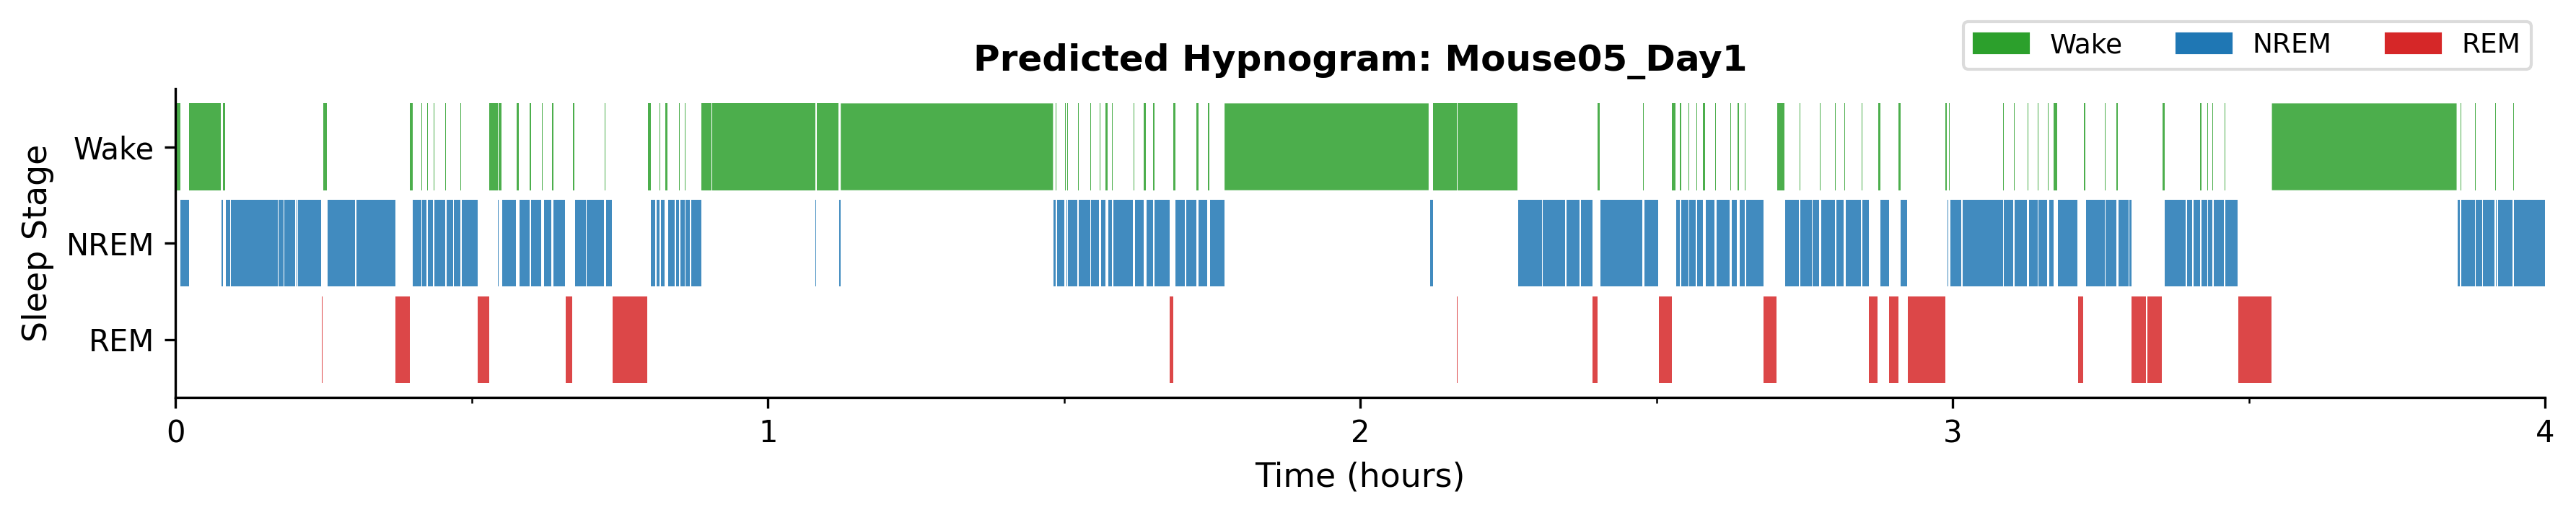
\includegraphics[width=\textwidth]{../figures/hypnograms/Mouse05_Day1_hypnogram.png}
  \caption{Predicted hypnogram: Mouse05, Day\,1.}
  \label{fig:hyp5}
\end{figure}

\begin{figure}[H]
  \centering
  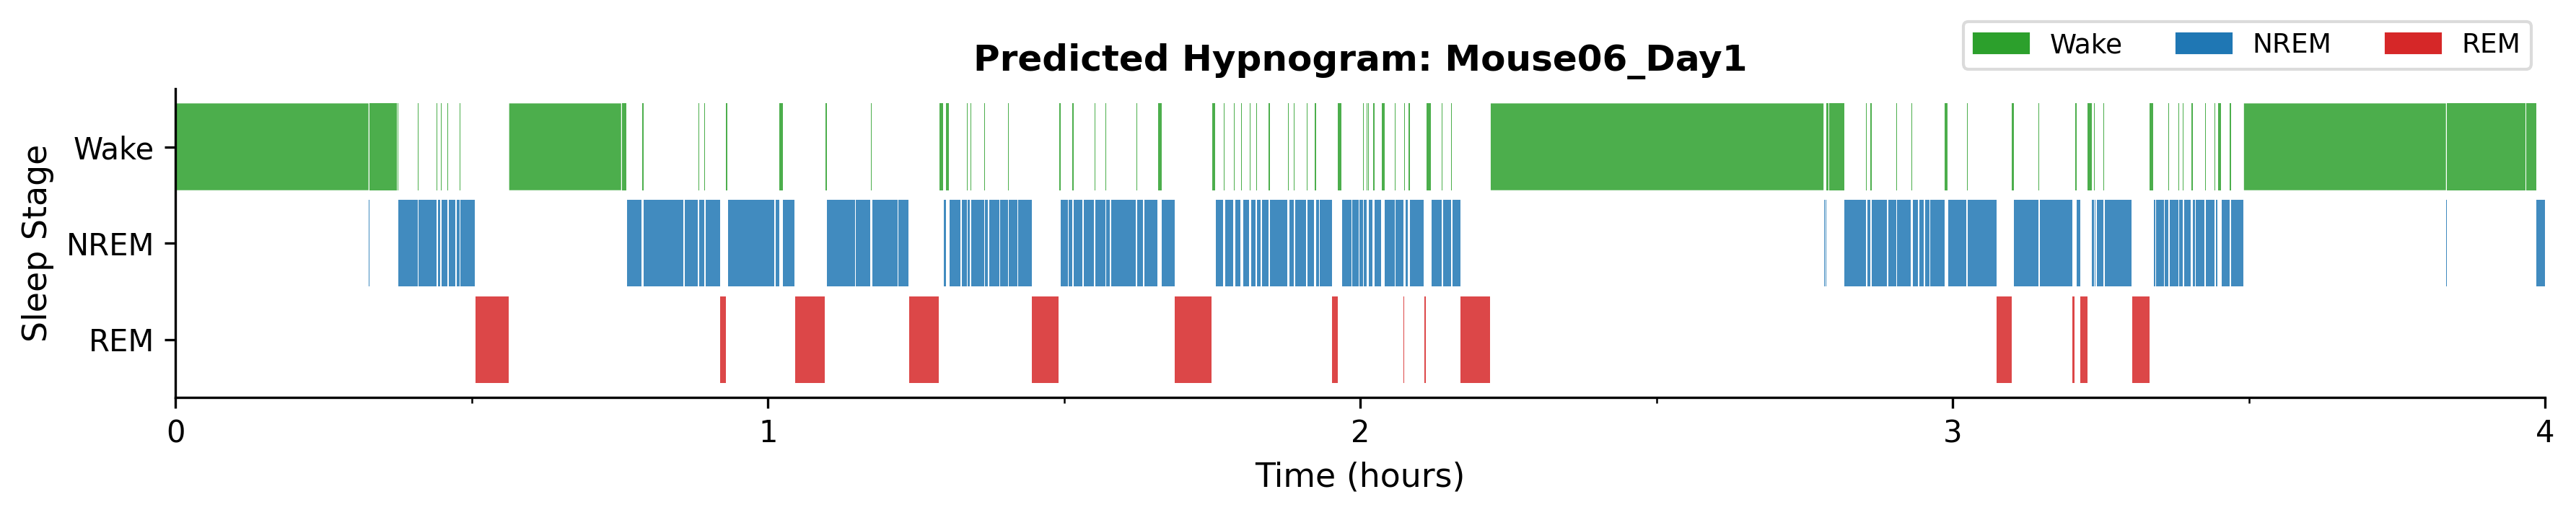
\includegraphics[width=\textwidth]{../figures/hypnograms/Mouse06_Day1_hypnogram.png}
  \caption{Predicted hypnogram: Mouse06, Day\,1.}
  \label{fig:hyp6}
\end{figure}

% ============================================================
\section{Limitations}
% ============================================================

\begin{itemize}
  \item This analysis uses the standard single-channel cortical EEG and nuchal
    EMG configuration for which AccuSleePy was designed and validated. Model
    performance may differ for non-standard electrode configurations or
    multi-region recording setups.
  \item All analyses are descriptive. Stage proportions, bout structures, and
    transition probabilities characterize what the data show. Biological
    interpretation of these results is the responsibility of the researcher; no
    mechanistic claims are made here.
  \item No recordings were excluded from the analysis. Flagged recordings (none
    in this dataset) are noted in \texttt{QC\_report.md} and Section~3.2 but
    remain included in all reported metrics. The decision to exclude any recording
    based on QC findings is left to the researcher.
  \item The validation comparison to expert manual labels is included as a
    technical quality check confirming correct pipeline execution. It is not
    intended to be interpreted as a primary scientific result of this analysis.
\end{itemize}

% ============================================================
\section{References}
% ============================================================

\begingroup
\renewcommand{\section}[2]{}  % suppress auto-section heading from natbib
\bibliographystyle{plainnat}
\begin{thebibliography}{9}

\bibitem[Barger et~al.(2019)]{Barger2019}
Barger, Z., Frye, C.\,G., Liu, D., Dan, Y., \& Bouchard, K.\,E. (2019).
Robust, automated sleep scoring by a compact neural network with distributional
shift correction.
\textit{PLOS ONE}, 14(12), 1--18.
\url{https://doi.org/10.1371/journal.pone.0224642}

\bibitem[Barger and Frye(2025)]{BargerOSF2025}
Barger, Z., \& Frye, C. (2025, June 6).
AccuSleep.
\url{https://doi.org/10.17605/OSF.IO/PY5EB}

\end{thebibliography}
\endgroup

\end{document}
